\documentclass{beamer}


% Load essential packages
\usepackage{hyperref} % Only load once to avoid conflicts
\usepackage{stile}
\usepackage{xcolor}
\usepackage{subcaption}
\usepackage{tcolorbox}
\usepackage[font=scriptsize,skip=1pt]{caption}
\usepackage[T1]{fontenc}
\usepackage{csquotes}
\usepackage[backend=biber, style=authoryear, maxnames=3, minnames=1, abbreviate=false, date=long, url=false, isbn=false, doi=false]{biblatex}
\addbibresource{lecture3/bib.bib} % Ensure this matches your bibliography file name

\interfootnotelinepenalty=10000

\usepackage{latexsym, amsmath, xcolor, multicol, booktabs, calligra}
\usepackage{graphicx, pstricks, listings, stackengine}

% Hyperref setup
\hypersetup{
    hidelinks,
    colorlinks=true,
    linkcolor=black,
    citecolor=deepblue,
    urlcolor=black
}

% Font theme for Beamer
\usefonttheme[onlymath]{serif}

% Custom definitions
\def\cmd#1{\texttt{\color{red}\footnotesize $\backslash$#1}}
\def\env#1{\texttt{\color{blue}\footnotesize #1}}
\definecolor{deepblue}{rgb}{0,0,0.5}
\definecolor{deepred}{rgb}{0.6,0,0}
\definecolor{deepgreen}{rgb}{0,0.5,0}
\definecolor{halfgray}{gray}{0.55}
\definecolor{deepgreen}{RGB}{29, 126, 44}

% Beamer color settings
\setbeamercolor{block title}{bg=blue!70!white, fg=white}
\setbeamercolor{block body}{bg=blue!10!halfgray, fg=white}
\setbeamercolor{section in head/foot}{fg=white}
\setbeamercolor{subsection in head/foot}{fg=white}
\setbeamercolor{title in head/foot}{fg=white}


% Listings settings for code highlighting
\lstset{
    basicstyle=\ttfamily\small,
    keywordstyle=\bfseries\color{deepblue},
    emphstyle=\ttfamily\color{deepred},
    stringstyle=\color{deepgreen},
    numbers=left,
    numberstyle=\small\color{halfgray},
    rulesepcolor=\color{red!20!green!20!blue!20},
    frame=shadowbox,
}

\author{Freya Rubel}
\title{Trade, Migration and Global Challenges}
\subtitle{Trade and the Environment}
\institute{}
\date{06.11.2025}

\graphicspath{{lecture3/}}

\begin{document}

\begin{frame}
    \titlepage
\end{frame}

\begin{frame}
    \tableofcontents[sectionstyle=show, subsectionstyle=show/shaded/hide, subsubsectionstyle=show/shaded/hide]
\end{frame}

\section{Trade and Deforestation}
\begin{frame}{Channels} 
    \begin{itemize}
        \item Specialization in agriculture (Export-oriented agriculture: palm oil, soy, beef, and timber) % we just learned about the comparative advantage. 
        \item Forest clearing for cattel ranch, plantations, mining etc.
        \item Infrastructure development % this could be railways, harbors, anything related to transport infrastructure that is required for trading across long distances
        \item Urbanization and economic growth % urbanization goes hand in hand with a more specialized society. 
        \item Carbon offset markets can conserve or expand forest cover
        % examples: fly and offset your carbon emissions by donating to this rainforest conservation initiative or that reforestation measure
        % Carbon offset markets enable companies or private consumers to purchase offsets from projects that reduce or sequester carbon, such as reforestation or forest conservation initiatives. 
        % These initiatives are oftentimes happening in countries of the global south and the service is offered to consumers in the global north trying to get a clean conscience about their own consumption choices 
        % this is a trade in service that is either conserving or expanding forest cover
    \end{itemize}
\end{frame}

\begin{frame}{Empirical Evidence}
\begin{itemize}
    \item \textcite{Alix-Garcia_Walker_Radeloff_Kozak_2018} study the effect of the 1850 Austro-Hungary customs union on deforestation. \pause
    % Do word customs union appeared briefly in last weeks lecture. Do you remember what a customs union is?
    % bilateral or multilateral trade agreement that is reducing or eliminating tariffs for the members of the customs union
     % this customs union was established when Hungary was formally incorporated into the Austrian Empire
    \item The authors assume that Hungary had a comparative advantage in agricultural production while Austria had a comparative advantage in manufactured goods.
    \item They find that the customs union led to a causal increase in cropland in Hungary by 8\% annually in the five years after establishment of the customs union. 
    \item At the same time, forest cover in Hungary decreased by 6\%.
    \item Due to data limitations for the Austrian sample post 1850, the authors can only offer suggestive evidence for a decrease in agriculture land in Austria after 1850.
\end{itemize}
\end{frame}

\section{Trade and Biodiversity}

\begin{frame}{Channels}
\begin{itemize} \small
    \item Land use and habitat change % similar to deforestation, a specialization in agricultur is changing the natural environment. Manufacturing on the other hand can go hand in hand with chemicals and air pollutants that threaten biodiversity
    \item Intensified agriculture (monocultures, pesticide use)
    % only one type of crop is planted on a field for an extended period of time and that obviously limits biodiversity because the human doesn't want diversity in plants but the side effect is that it also limits the diversity of animals that live in these fields and in the soil
    \item Pollution and chemicals from manufacturing
    \item Climate Change % fueled by economic growth
    \item Introduction of invasive species % ship trade is introducing foreign species into new regions of the world
\end{itemize}    
\end{frame}

\begin{frame}{Some Evidence on Channels}
    \begin{itemize} \small
        \item In 2011, an estimated 33\% of Central and Southern America and 26\% of Africa’s biodiversity losses were driven by consumption in other world regions (\cite{marques2019increasing})
        \item Plastic pollution has been identified as one of the top threats to the extent of all living beings and their variety, especially in the marine context (\cite{marine_biodiversity}). % waste trade
        \item Projections on the magnitude of biodiversity loss vary hugely (\cite{biodiversity_review}) but one of the earliest global studies estimated that by 2050 15-37\% of species are thought to go extinct under intermediate climate warming (\cite{thomas_extinction_2004}).
        \item Invasive species are the sole driver of 16\% of documented global animal and plant extinctions (\cite{ipbes2023invasive}).
    \end{itemize}
\end{frame}

\begin{frame}{Relevance}
    \Large \textbf{Why do economists care about biodiversity?}
    % I didn't ask this question earlier because I think trees and forests are easier to grasp
\end{frame}

\begin{frame}{Biodiversity, Financial Stability, and Economic Wellbeing}
    \begin{itemize} \small
    \item All companies depend on ecosystem services, such as clean air, fresh water, fertile soils and a stable climate, to varying degrees.
        \item \textbf{Biological insurance:} A diverse ecosystem is less vulnerable to external shocks and provides a buffer to times of crisis (\cite{Loreau2021}).
        \item  Some researchers estimated ecosystem services to contribute more than twice as much to human well-being than global GDP (\cite{COSTANZA_ecosystem_services}).
        \item \textcite{COSTANZA_ecosystem_services} estimate the loss of ecosystem services between 1997-2011 due to land use change at around 10 trillion\$ per year
       \item Financial institutions, especially the European Central Bank (ECB) and the Banque de France are concerned with the loss of biodiversity for financial stability. 
       \item[\href{https://www.youtube.com/watch?v=DP3tRzELPLY}{\textcolor{deepblue}{\underline{Link:}}}] \textit{\footnotesize ECB Podcast - What biodiversity and nature loss mean for our economy} 
    \end{itemize}
\end{frame}

\section{Trade and Carbon Emissions}
% this is where we left off. Trade and Carbon Emissions

\begin{frame}{Consumption vs. Production based CO2 emission - US}
    \begin{figure}
        \centering
        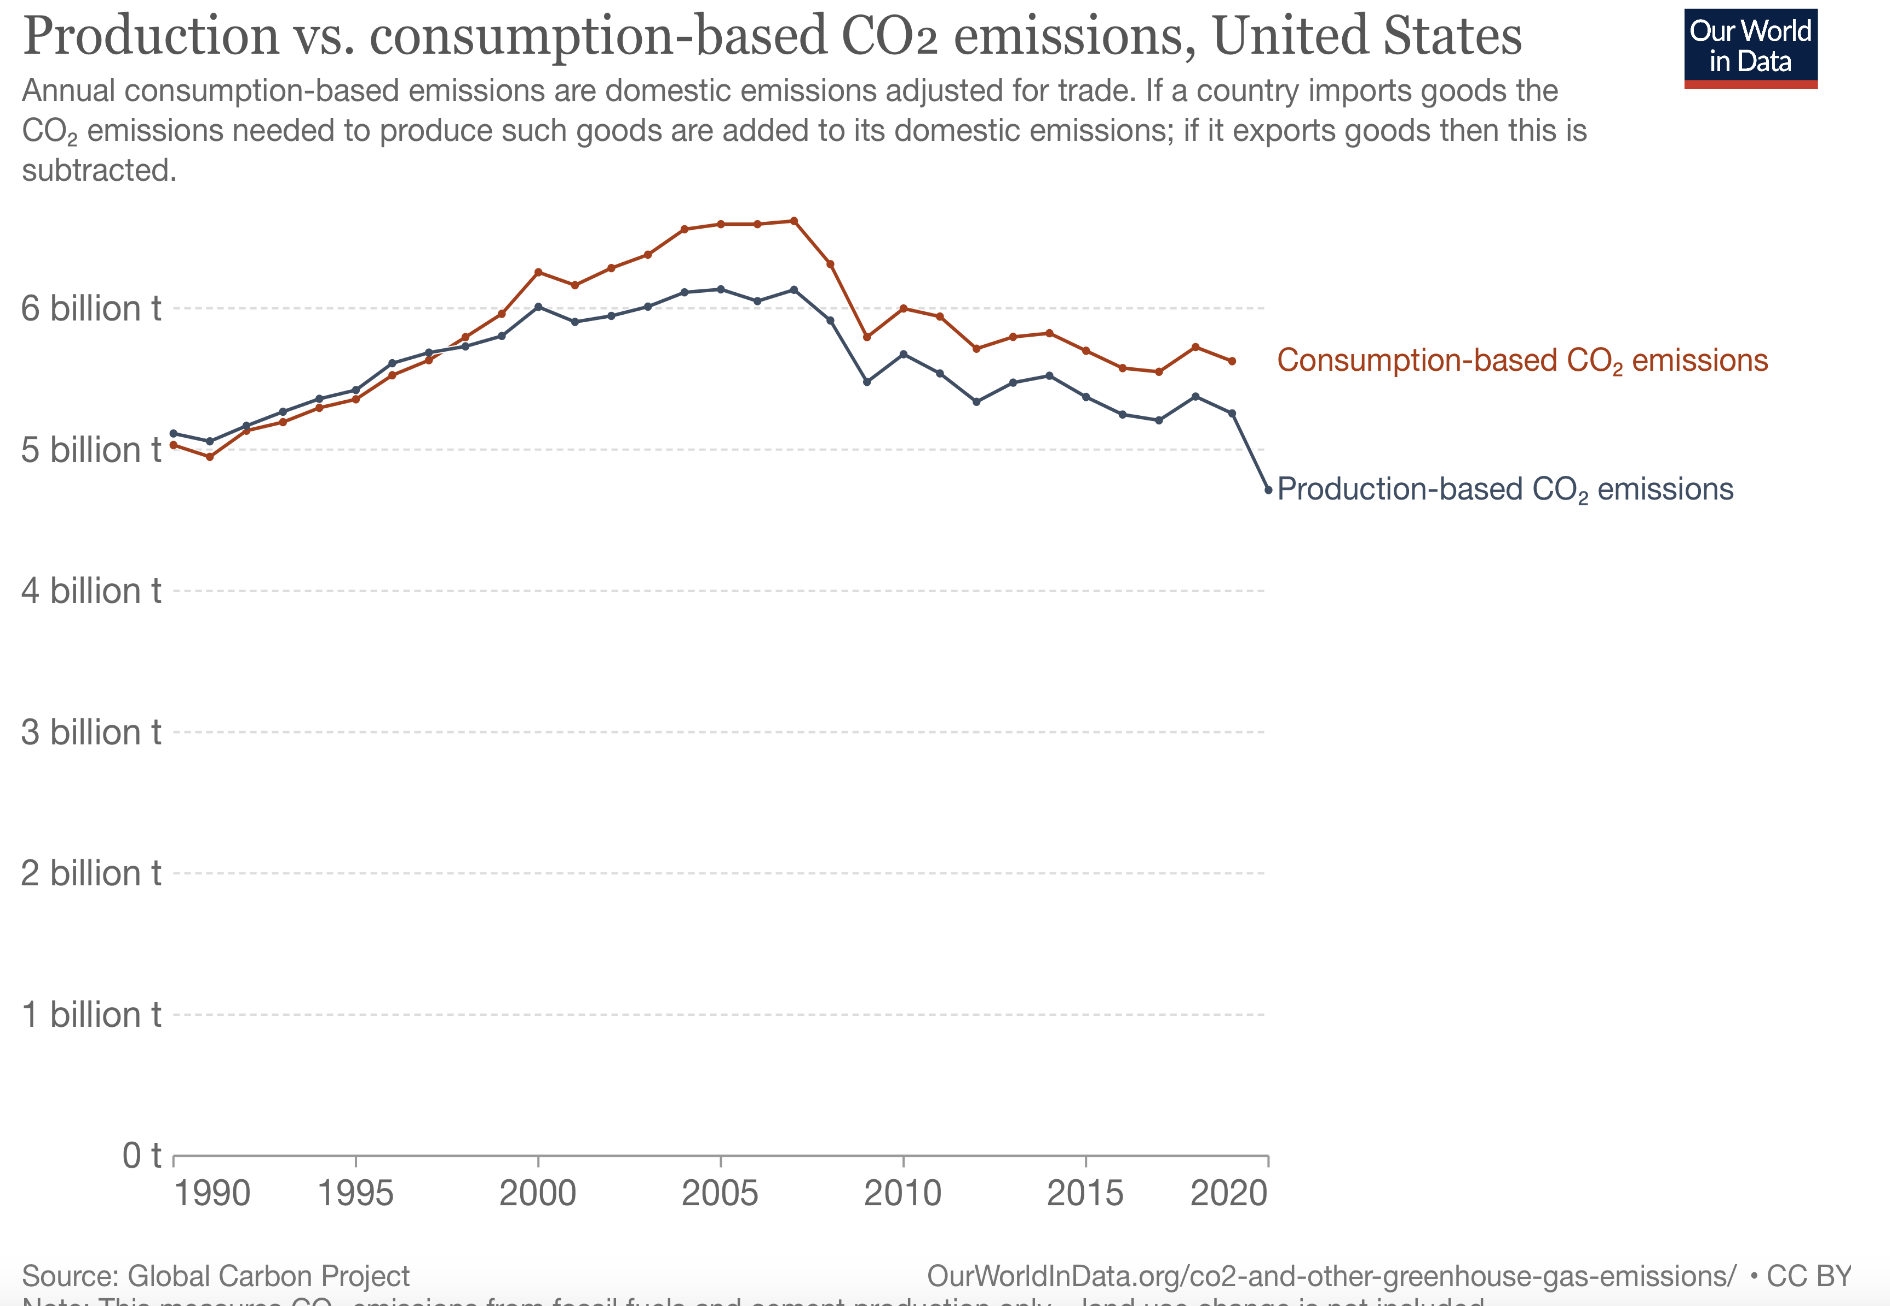
\includegraphics[width=0.8\linewidth]{co2 emissions us.png}
        \caption{United States consumption vs. production based CO2 emission}
        \label{fig:enter-label}
    \end{figure}
\end{frame}

\begin{frame}{Consumption vs. Production based CO2 emission - France}
    \begin{figure}
        \centering
        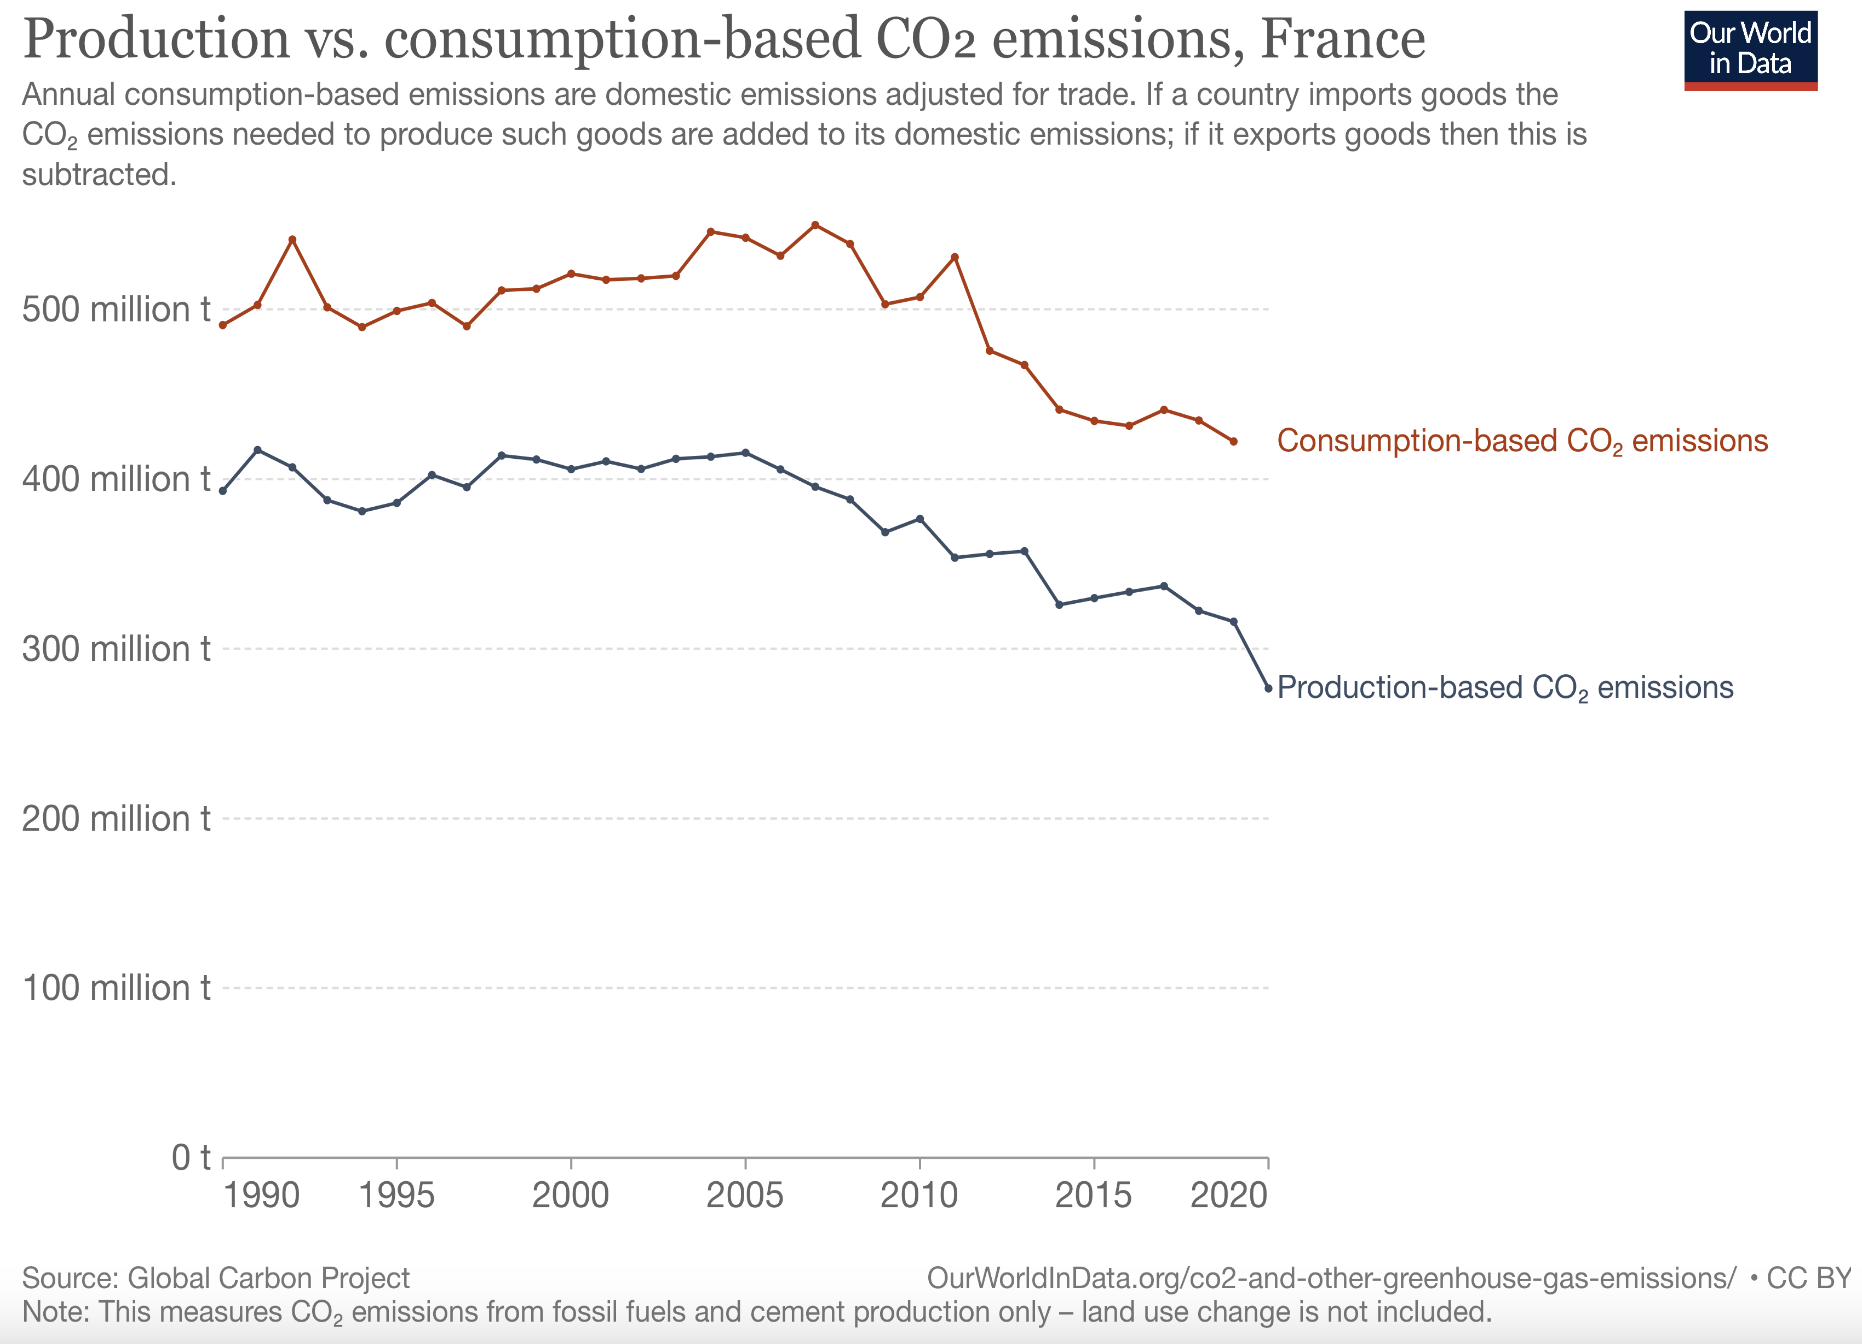
\includegraphics[width=0.8\linewidth]{co2 emissions france.png}
        \caption{France consumption vs. production based CO2 emission}
        \label{fig:enter-label}
    \end{figure}
\end{frame}

\begin{frame}{Consumption vs. Production based CO2 emission - China}
    \begin{figure}
        \centering
        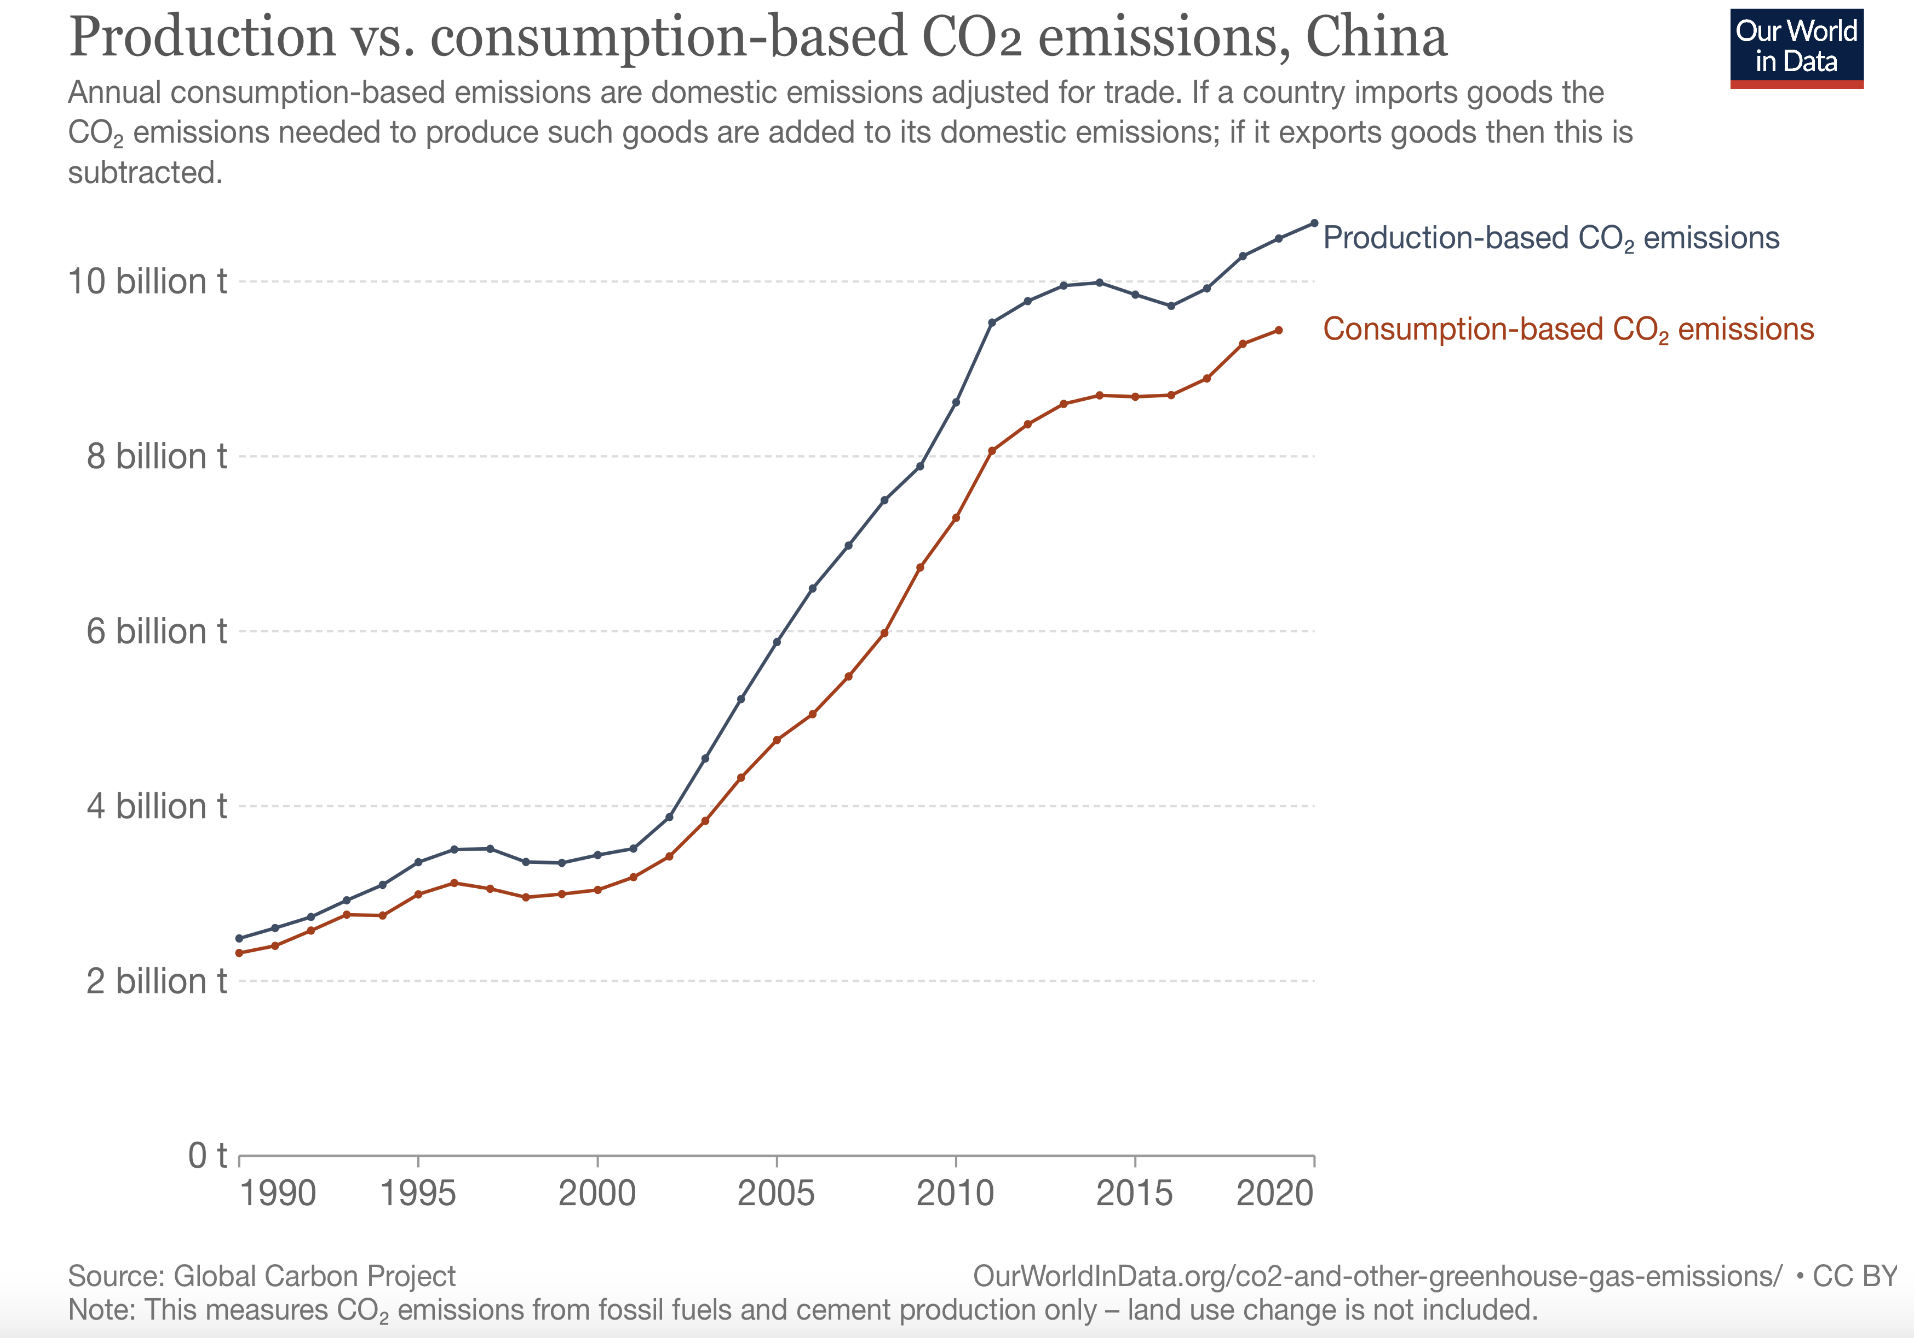
\includegraphics[width=0.8\linewidth]{co2 emissions china.png}
        \caption{China consumption vs. production based CO2 emission}
        \label{fig:enter-label}
    \end{figure}
\end{frame}

\begin{frame}{Consumption vs. Production based CO2 emission - India}
    \begin{figure}
        \centering
        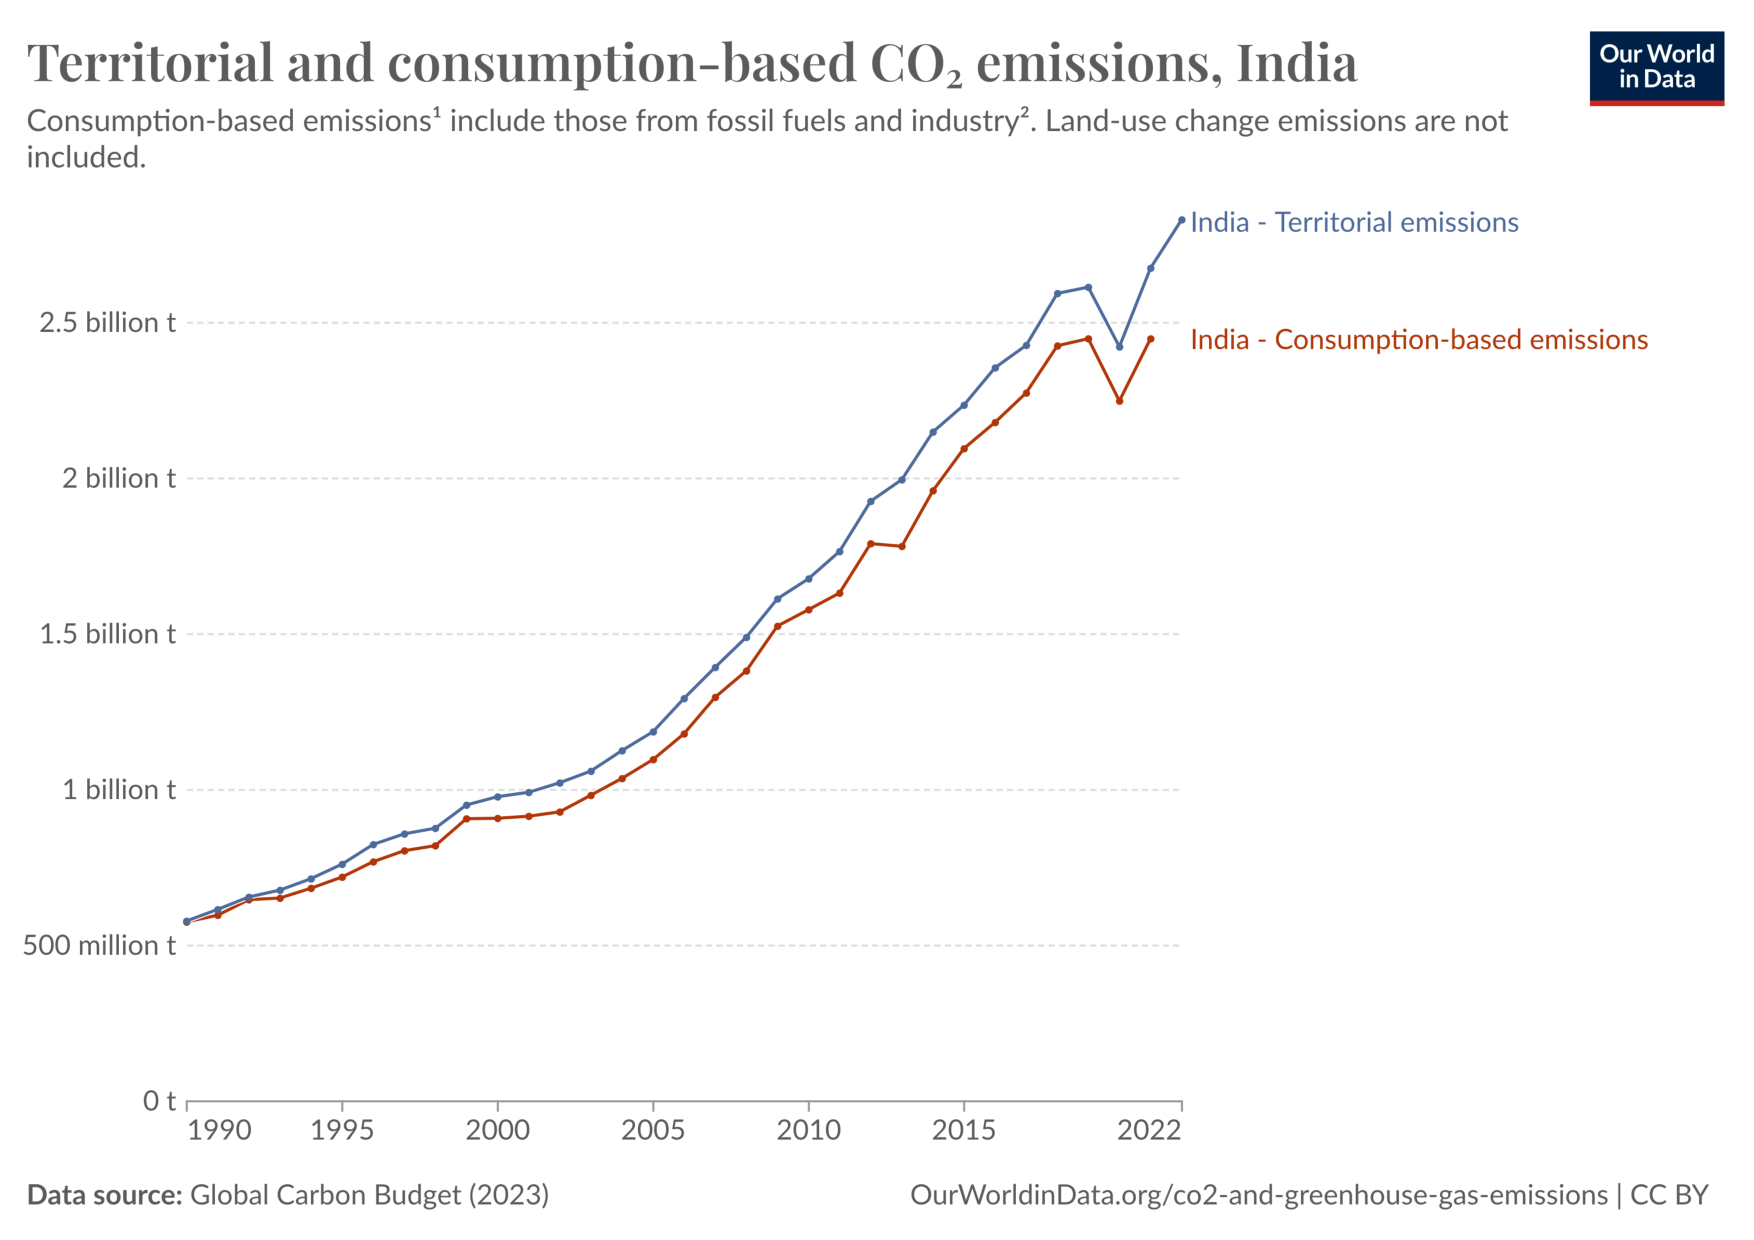
\includegraphics[width=0.8\linewidth]{co2 india.pdf}
        \caption{India consumption vs. production based CO2 emission}
        \label{fig:enter-label}
    \end{figure}
\end{frame}

\begin{frame}{Net Effect of Trade on Carbon Emissions}
    Is international trade good or bad for global emission levels? \pause \\
    \textbf{The debate is ongoing.} % it is very very hard to find an answer to this question. In economics, we are obsessed with causal effect. Correlations are not enough. Causality counts. We want to know the causal effect of trade on carbon emissions and it is almost impossible to do this
    \begin{itemize} \small
        \item International trade has led to economic growth, which is going hand in hand with carbon emissions. \textcolor{red}{$\blacktriangle$}
        \item Trade of goods is associated with emissions from transport. \textcolor{red}{$\blacktriangle$}
        \item The trade has also led to the diffusion (spillover effects) of technology, which is decreasing the environmental impact of production. \textcolor{deepgreen}{$\blacktriangledown$}
        \begin{itemize} \footnotesize
             \item If production were to take place where the carbon footprint is comparatively lower, international trade holds the potential to decrease global emissions. The idea is called the green comparative advantage.
        \end{itemize}
        \item Trade agreements are increasingly incorporating environmental standards, which can accelerate the decarbonization. \textcolor{deepgreen}{$\blacktriangledown$}
    \end{itemize}
\end{frame}

\section{Emission Trading Systems}

\begin{frame}{Emission Trading System (ETS)}
    \textbf{Principle of the ETS:} \\
    The Emission Trading System (ETS) is a market-based approach to reduce greenhouse gas emissions by setting a cap on total emissions. Companies receive or buy permits (allowances) to emit. They can trade these permits once bought/allocated to them. \vspace{0.3cm}

    \textbf{Two Main Initial Permit Distribution Methods:}
    \begin{itemize}
        \item \textbf{Grandfathering} (Free Allocation): Permit allocation based on historical emissions.
        \item \textbf{Auctioning}: Permits sold to the highest bidder, reflecting market value.
    \end{itemize}
\end{frame}

\begin{frame}{The EU Cap-and-Trade System}
    \begin{itemize}
        \item The EU ETS, established in 2005, is the world's largest carbon market, aiming to reduce greenhouse gas emissions by setting a cap on emissions for certain industries and power sectors.
        \item It operates on a "cap-and-trade" principle: a cap is set on total emissions, and emission allowances (permits) are distributed to firms, who can trade these permits.
        \item Firms that reduce emissions below permits can sell excess permits, while those exceeding their limits must buy additional permits or face penalties.
    \end{itemize}
\end{frame}

\begin{frame}{Phases of the EU ETS and Permit Allocation}
    \begin{enumerate}
        \item \textbf{Phase 1 (2005–2007)}: 
            \begin{itemize}
                \item Goal: Establish a functioning carbon market.
                \item Permit Allocation: Permits were given out for free based on historical emissions (grandfathering).
                \item Lessons Learned: Over-allocation led to a surplus of permits, and low permit prices reduced the incentive to cut emissions.
            \end{itemize}
        
        \item \textbf{Phase 2 (2008–2012)}: 
            \begin{itemize}
                \item Goal: Align with the Kyoto Protocol targets (specific emission reduction targets).
                \item Permit Allocation: Slightly fewer free permits, with auctioning introduced for some sectors.
                \item Lessons Learned: Improved regulation reduced over-allocation, but the economic recession caused another surplus and kept prices low.
            \end{itemize}
    \end{enumerate}
\end{frame}

\begin{frame}{Phases of the EU ETS and Permit Allocation (continued)}
    \begin{enumerate}
        \setcounter{enumi}{2}
        \item \textbf{Phase 3 (2013–2020)}: 
            \begin{itemize}
                \item Goal: Increase market stability.
                \item Permit Allocation: Significant increase in auctioning (50\% of permits), and allocation was based on EU-wide benchmarks rather than historical emissions.
                \item Lessons Learned: Prices rose due to tighter caps and the Market Stability Reserve (MSR) was introduced to reduce permit surplus.
            \end{itemize}
        
        \item \textbf{Phase 4 (2021–2030)}: 
            \begin{itemize}
                \item Goal: Strengthen the EU ETS to meet the EU's 2030 climate targets.
                \item Permit Allocation: Auctioning is the default, with free allocation only for certain sectors.
            \end{itemize}
    \end{enumerate}
\end{frame}

\begin{frame}{Determinants of the Carbon Permit Price}
\textbf{Supply}: Number of permits allocated onto the market (cap)
    \begin{itemize}
        \item Market Stability Reserve (MSR): mechanism designed to address imbalances in supply and demand for allowances. Absorbs excess allowances from the market when there's an oversupply and releases allowances if there's a shortage.
    \end{itemize}
\textbf{Demand}: Number of permits demanded by producing firms
    \begin{itemize}
        \item Production levels (state of the economy)
        \item Technological advancements
        \item Energy prices (fuel switching)
        \item Scaling up of renewable energy generation
        \item Anticipation effects
    \end{itemize}
%On the demand side, we need to think about which firms need permits and why that demand changes over time.
%Production levels are straightforward — when the economy grows, industrial output increases, more electricity is consumed, and firms need more permits to cover their emissions. During recessions, the opposite happens. This is why permit prices often track economic cycles.
%Technological advancements affect demand in two ways. First, if firms adopt cleaner production processes or install carbon capture equipment, they emit less per unit of output and need fewer permits. Second, improvements in energy efficiency mean less fuel consumption for the same production level, again reducing permit demand. The EU ETS creates an incentive for these investments because reducing emissions becomes financially valuable.
%Energy prices matter because of fuel switching — particularly in electricity generation. When natural gas prices are low relative to coal, power plants switch from coal to gas. Since gas emits roughly half the CO₂ per unit of energy, this shift substantially reduces permit demand. The reverse happens when gas becomes expensive. This mechanism links the carbon market directly to fossil fuel markets.
%Renewable energy scaling reduces permit demand mechanically. Every megawatt-hour generated by wind or solar displaces fossil fuel generation that would have required permits. As renewables become cheaper and their capacity expands, fewer permits are needed to meet electricity demand. This is a structural force pushing demand downward over time.
%Anticipation effects introduce a forward-looking element from the firm's perspective. If firms expect permit prices to rise — perhaps due to a planned cap reduction — they may buy and bank permits now rather than later, increasing current demand. Conversely, if policy uncertainty makes firms think the system might weaken, they may delay purchases, suppressing current demand. This makes the permit price partially a reflection of expectations about future policy stringency.
\end{frame}

\begin{frame}{Carbon Permit Price per Tonne of CO2 Emitted}
    \begin{figure}
        \centering
        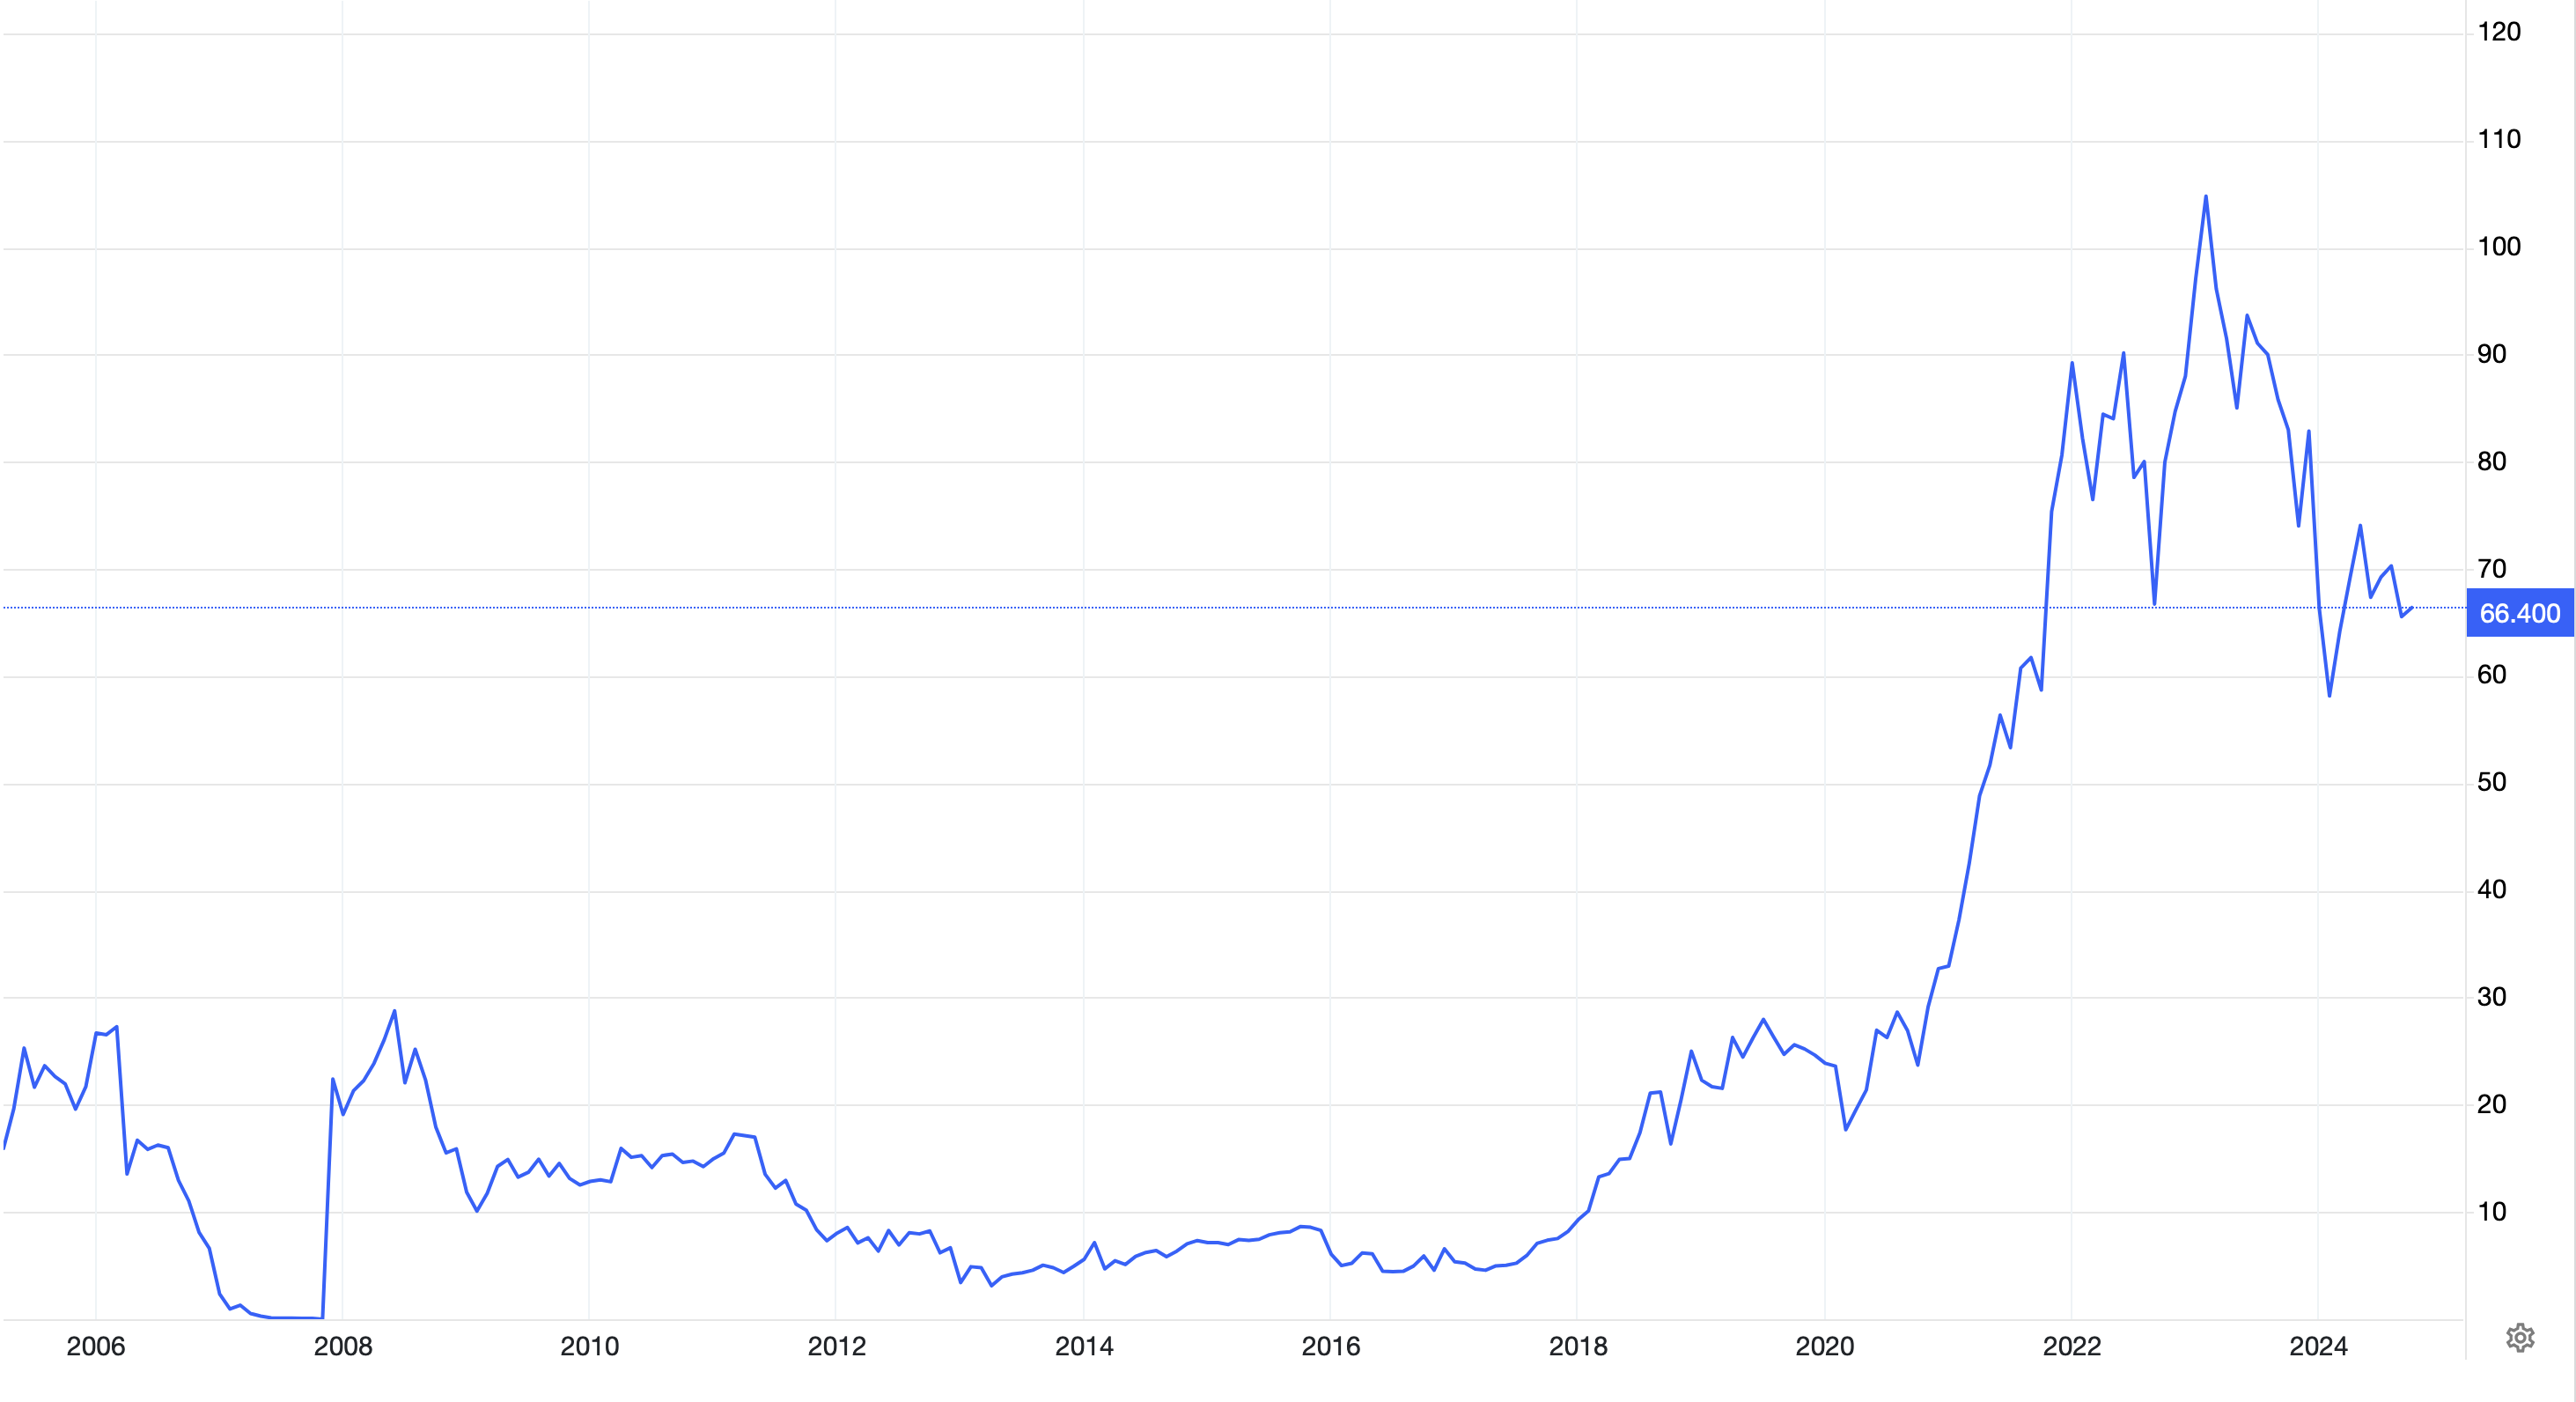
\includegraphics[width=\linewidth]{carbon_permit_price.png}
        \caption{Price (EUR) per tonne of CO2 emitted between 2005 and 2024. Source: \textcite{tradingeconomics2024carbon}}
        \label{fig:enter-label}
        % please describe this graph
        % 2008-2017:  prices first dropped and then stabilized at a low level below €10 tCO 
        %% financial crises reduced economic activity and with that the emission of carbon 
        %% for many years, the ETS failed at the most basic thing: establishing a price for carbon that is hurting producers enough in order to drive decarbonization (investment in alternative technology that needs less carbon)
        % 2018-2020: the first rise up to a plateau of €20–30 tCO2 
        %% economic actors switched from short-sight to long-sight planning horizons
        % late 2020 stark increase and somewhere between 70-90 tCO2
    \end{figure}
\end{frame}

\begin{frame}{Shortcomings of the EU ETS}
    \begin{itemize} \small
        \item Persisting concern about carbon leakage and economic competitiveness: the risk that production gets relocated to countries with less stringent climate policies.
        \item Sectoral limitations: In 2022, the ETS covered emissions representing around \textbf{37\% of the EUʼs total emissions} (\cite{eea2023ghg}). 
        \item Volatile prices make for an unstable investment environment for businesses
        \item Limited effect on consumer behaviour, lack of visibility
        \item Regional disparities in impact because of sectoral division across member states
    \end{itemize}
\end{frame}

\begin{frame}{Introduction to the Carbon Border Adjustment Mechanism (CBAM)}
    \begin{itemize} \small
        \item The EU's Carbon Border Adjustment Mechanism (CBAM) is a policy tool designed to address carbon leakage.
        \item Up until now, sectors where emissions are high and global competition is strong (Emission Intensive Trade Exposed (EITE) industries) have been exempt from the EU ETS because of a fear of carbon leakage.
        \item CBAM is set to impose a carbon price on imported goods from countries without equivalent carbon pricing, as well as European industries, levelling the playing field for EU and non-EU producers.
        \item Gradual inclusion of the EITE producers into the EU carbon market from 2026 to 2034.
    \end{itemize}
\end{frame}

\begin{frame}{Impact on Carbon-Intensive and Trade-Exposed Industries}
    \begin{itemize}
        \item Non-EU exporters to the EU will need to purchase CBAM certificates, effectively paying for the carbon content of their products, similar to EU firms under the ETS.
        \item In theory, this policy should encourage foreign industries to adopt cleaner practices to remain competitive in the EU market, aligning them with EU climate objectives.
        \item The price is deductible for producers in countries or regions in which a carbon price is already being paid (to avoid double-taxation).
    \end{itemize}
\end{frame}

\begin{frame}{Implications and Challenges for Global Trade}
    \begin{itemize}
        \item For EITE industries outside the EU, CBAM could increase costs and necessitate investment in low-carbon technologies to maintain market access to the EU.
        \item CBAM may drive countries with less stringent climate policies to adopt stronger carbon measures to capture the money paid in carbon tax/tariff. % if the domestic producers need to pay for their carbon content anyways, better make it their home countries so that states can get some tax revenues
        \item Challenges remain: potential for trade disputes, technical complexity in measuring carbon content, and justice concerns $\rightarrow$ Should we hold steel producers in India to the same environmental standards as steel producers in Finland?
    \end{itemize}
\end{frame}

\begin{frame}{Paper on $NO_x$ Emission Trading Program}
\begin{center}
    \begin{Large}
        \textbf{What Do Emissions Markets Deliver and to Whom? Evidence from Southern California's $NO_x$ Trading Program} \vspace{0.2cm}\\
    \end{Large} 
    by Meredith Fowlie, Stephen P. Holland, and Erin T. Mansur \\
    published in American Economic Review, vol. 102, no. 2, April 2012
\end{center}
\end{frame}

\begin{frame}{Southern California’s $NO_x$ Trading Program}
\textbf{Background} \\
\begin{itemize}
    \item Los Angeles suffers from some of the worst air quality in the United States. 
    \item In 1994, the South Coast Air Quality Management District introduced a market-based emission trading system: the REgional CLean Air Incentives Market (RECLAIM). \\
    \item RECLAIM covers 392 facilities whose combined $NO_x$ emissions accounted for over 65\% of the region’s $NO_x$ emissions. % sources emitting less than 4 tonnes per year were omitted 
    \item $NO_x$ (nitrogen oxides) are non-uniformly mixing pollutants. % it means that in contrast to CO2, which is warming the planet no matter where it is emitted, NOx is hurting the environment where it is locally emitted
\end{itemize}
\end{frame}

\begin{frame}{Motivation of the Paper}
    \begin{itemize}
        \item Need to evaluate if emissions trading (market-based regulation) can achieve significant reductions compared to traditional command-and-control (CAC) regulations. % simply tell companies that they cannot 
        \item Questions of environmental justice, particularly distributional impacts on minority and low-income communities, are central to evaluating RECLAIM's efficacy and fairness since we don't solely care about the level of emissions, but also about where they arise.
    \end{itemize}
\end{frame}

\begin{frame}{How the RECLAIM Market Works}
    \begin{itemize}
        \item RECLAIM allocates emissions permits to facilities in the Los Angeles area, allowing them to trade permits within a regulated cap.
        \item Initial allocation of permits was based on historical emissions (grandfathering), creating flexibility for facilities to either reduce emissions or trade for additional permits.
        \item Aim: replace existing CAC regulations while achieving similar or greater reductions in $NO_x$ emissions.
    \end{itemize}
\end{frame}

\begin{frame}{Empirical Strategy}
    Main Challenge: To estimate the causal effect of this policy, one needs to credibly identify a \textbf{counterfactual}. \pause
    \begin{itemize}
        \item \cite{california_nox} exploit the fact that some factories were exempt from the new RECLAIM regulation and continued to work under the CAC regime.
        \item The authors match each factory under the RECLAIM program to one factory that is closest in a number of characteristics (nearest-neighbor matching).
        \item The authors assume that - in the absence of the new program - factories would have followed the same trend as their matched factory $\rightarrow$ this allows them to estimate the emission levels of the factories in the absence of the new program.
    \end{itemize}
\end{frame}

\begin{frame}{Key Results of the Paper}
    \begin{itemize}
        \item Emissions at RECLAIM facilities decreased by approximately 25\% relative to CAC facilities.
        \item \cite{california_nox} do not find any evidence that supports the hypothesis that the relative effects of RECLAIM on facility-level emissions vary systematically with neighbourhood demographic characteristics like income or racial composition. % one of the big concerns of opponents of the regulation: Emissions would get traded to neighborhoods with less influence and power 
    \end{itemize}
\end{frame}

\begin{frame}{Discussion and Limitations of the Paper}
    \begin{itemize}
        \item Between periods 1 and 4 of the program, approximately 32\% of RECLAIM facilities and nearly 54\% of non-RECLAIM facilities do not submit emissions reports for one or several years.
        \item Even though the authors are explicitly interested in the geographic source of the emission, they do not discuss that firms could have also located their production to other states with lower emission regulation (\textbf{leakage problem}).
        \item If a switch to the mandatory RECLAIM program had led to a considerable move of emissions from official RECLAIM facilities to other states (outside California), what would be the implication for the estimated effect ($25\%$ emission reduction) of a switch from CAC to Cap-and-Trade?
    \end{itemize}
\end{frame}

\section{References}
\begin{frame}[allowframebreaks]{References}
    \printbibliography
\end{frame}


\end{document}

